\section{Numerical Results and Discussion}
First, to check how do different groups evolve, we conducted this experiment
and presented the variation of these groups. Second, to verify its performance
and stability, the GA was run many times, the best, worst case, and average
results were presented. Finally, we compared the result with the work in the
other literature.

\begin{figure}[!htb]
	\centering
	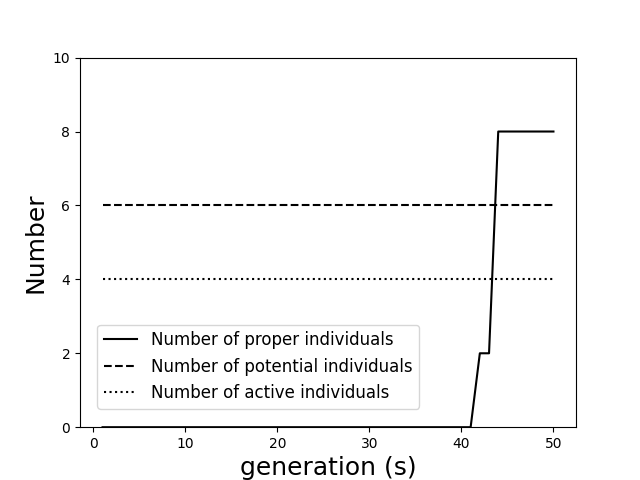
\includegraphics[width=\linewidth]{fig/group_number.png}
	\caption{Number of individuals in each group as a function of generation.}
	\label{fig:group}
\end{figure}

\begin{figure}[!htb]
	\centering
	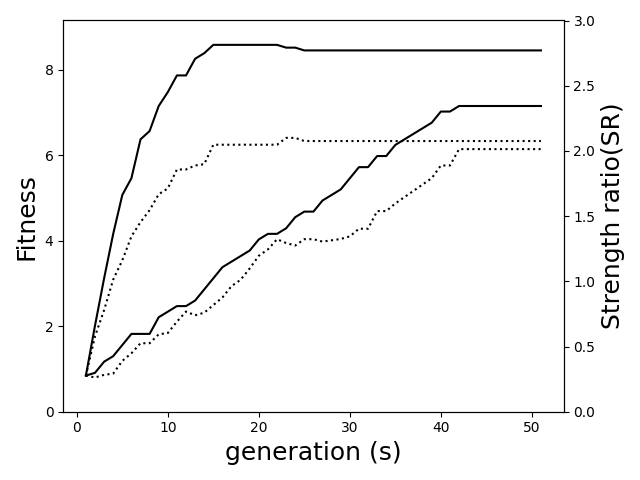
\includegraphics[width=\linewidth]{fig/fitness_strength_ratio.png}
	\caption{Fitness and strength ratio as a function of generations.}
	\label{fig:sr}
\end{figure}



Figure \ref{fig:group} shows the number of individuals in each group during
the one-time GA process.  For both active group and potential groups, the number of
individuals is to its upper bound from the beginning to the end of the
searching process. However, for the proper group, at the initial stage of GA,
no individual fulfills the constraint, so the number of proper individuals is
zero. As seen from figure \ref{fig:group}, after forty generations, proper
individuals appeared and increased very quickly to its number upper bound.


The GA process can be divided into two phases by whether there are individuals
that are appropriate or not. The figure \ref{fig:sr} shows the GA process in
which the dashed vertical line is the watershed between the initial phase and
the last phase. In the initial phase, no individual's strength ratio is over
the specified threshold; there are two approaches that GA could obtain a better
solution, though none of them are feasible, the first is increasing the length
of the chromosome, and the second is adjust the internal structure of a chromosome. So
in the first first stage, the fitness gets more and more smaller because the
increase of chromosome's length; however, at the point 1 on the fitness curve
of the GA, the fitness suddenly goes up due to the chromosome's adjustment; the
corresponding strength ratio of point 1 on the generation-strength ratio curve
is denoted by the point $1^{\prime}$, and its strength ratio goes up.  Then GA
comes to its second phase. During this phase, the GA already found proper
individuals which could satisfy the constraint, so the target in this stage is
to improve the fitness. This means GA needs to adjust its inner structure, at
the point 2 and 3 on the generation-fitness curve, the fitness curves went up,
and the corresponding strength ratio of these two points slightly went down,
but both of them still satisfy the constraint.


\begin{table*}
\caption{The optimum lay-ups for the loading $N_x=1e^6$ N when changing the value length mutation coefficient, the performance of the GA can be improved when the lenght mutation coefficient is reduced to 1.}
\centering
\begin{adjustbox}{width=1\textwidth}
	\begin{tabular}{cccccccc}
	\toprule
	coefficient		     &	 Material		               	 & case     & Stacking sequence    & Strength ratio  & Mass  &  Cost   & Layer    \\ 
	\midrule																															  
	\multirow{6}{*}{1} &	\multirow{3}{*}{glass-epoxy}   	 & worst     &  $[0_{80}/90_{52}]$ & 2.010           &  8.58  & 132     & 132   \\
						 &								     & best      &  $[0_{75}/90_{43}]$ & 2.000           &  7.67  & 118     & 118  \\
					     &									 & average   &    		           & 2.012           &  7.83  & 123     & 123  \\
						 &	\multirow{3}{*}{graphite-epoxy}	 & worst     &  $[0_{17}/90_{15}]$ & 2.036           & 1.68   & 80      & 32      \\
					     &								     & best      &  $[0_{17}/90_{5}]$  & 2.005           & 1.15   & 55      & 22      \\
					     &								     & average   &                     & 2.018           & 1.47   & 70      & 28      \\
	\multirow{6}{*}{5} &	\multirow{3}{*}{glass-epoxy}   	 & worst     &  $[0_{72}/90_{64}]$ &  2.009          & 8.84   &  136    &  136   \\
						 &								     & best      &  $[0_{72}/90_{53}]$ &  2.003          & 8.12   &  125    &  125   \\
					     &									 & average   &                     &  2.008          & 8.55   &  131    &  131  \\
						 &	\multirow{3}{*}{graphite-epoxy}	 & worst     &  $[0_{18}/90_{24}]$ &  2.006          & 2.20   &  105    &  42  \\
					     &								     & best      &  $[0_{17}/90_{6}]$  &  2.001          & 1.20   &  57     &  23  \\
					     &								     & average   &                    &   2.022          & 1.54   &  73     &  29  \\
	\bottomrule																															  
\end{tabular}
\end{adjustbox}
\label{tab:optimum_layup}
\end{table*}
            
            

Table \ref{tab:optimum_layup} shows the searching results after conducting this
experiment one hundred times in two different coefficient situations for
glass-epoxy and graphite-epoxy material, respectively. The best, worst, and
average experiment results are represented in this table. For the glass-epoxy
material, if the coefficient value takes 1, the best and worst sequences are
$[0_{80}/90_{52}]$, $0_{75}/90_{43}$, respectively; the average mass, cost, and
the number of layers are 1.68, 123, 123. However, if the coefficient takes a
relative bigger value, the performance of GA is better than the GA with a smaller
coefficient value. When the coefficient takes 1, the number of layers for the
best and worst cases are 118 and 132, respectively. When the coefficient value
si 5, the number of layer for them are 125 and 136, respectively. When
graphite-epoxy was taken as the experiment material, similar experiment
results were presented. This is because the mutation coefficient can control
both the convergence speed and search performance, a small mutation coefficient
would slow the convergence speed, however, it would lead to a small-grained
search in the local. 


\begin{table*}[!htb]
\caption{The optimum lay-ups for the loading $N_x=1e6$ N}
\centering
\begin{adjustbox}{width=1\textwidth}
\begin{tabular}{c|cc|cc}
	\toprule
	Cross Ply $[0_M/90_N]$         & \multicolumn{2}{c}{Previous Research} & \multicolumn{2}{c}{Current Research} \\
	\midrule																								  
	 Material       &  Glass-Epoxy & Graphite-Epoxy  & Glass-Epoxy & Graphite-Epoxy      \\ 
	      M         &  68          &    17           &  78		    &  18             \\
	      N         &  72          &    18           &  28		    &  8              \\
no. of lamina(n)    &  140         &    35           &  106	    &  26                     \\
         SR         &  2.01        &    2.10         &  2.03	    &  2.16            \\
     weight         &  9.10        &    1.84         &  6.89	    &  102.5           \\
	\bottomrule
\end{tabular}
\end{adjustbox}
\label{tab:comparsion}
\end{table*}

Table \ref{tab:comparsion} shows the optimal lay-up sequences by the variant GA
and  Choudhury and Mondal's\cite{choudhury2019failure} study. For the loading
case $Nx=1$ MPa m, the optimal lay-ups are a $[0_{68}/90_{72}]$  cross ply
laminate if glass-epoxy are taken, however,  in the present study, a
$[0_{78}/90_{28}]$ glass-epoxy cross ply laminate has been found which
significantly reduces both the cost and weight with increasing laminate's SR;
If graphite-epoxy was used, compared with the $[0_{17}/90_{18}]$ cross ply
laminate, an alternative cross ply laminate is found, its lay-up is $[0_{18}/90_8]$.
